\section{24 - MAT - AN 1.1, FA 2.2, FA 5.2, FA 5.3, FA 5.6, WS 1.1, WS 1.2 - Bevölkerungsentwicklung - BIFIE Aufgabensammlung}

\begin{langesbeispiel} \item[0] %PUNKTE DES BEISPIELS
				Die Weltbevölkerung ist in den vergangenen Jahrhunderten unterschiedlich stark gewachsen. Für die weitere Entwicklung bis zum Ende dieses Jahrhunderts gibt es unterschiedliche Prognosen.
				
				Abbildung 1 zeigt die Bevölkerungsentwicklung in den vergangenen 3\,000 Jahren.\\			
				Abbildung 2 zeigt die Bevölkerungsentwicklung von 1750 bis 2010.\\				
				Abbildung 3 zeigt die Bevölkerungsentwicklung von 1950 bis 2010.
				
				Die untenstehende Tabelle zeigt die Bevölkerungsentwicklung nach Kontinenten und Subkontinenten von 1900 bis 2000.
				
				\begin{center}\resizebox{0.6\linewidth}{!}{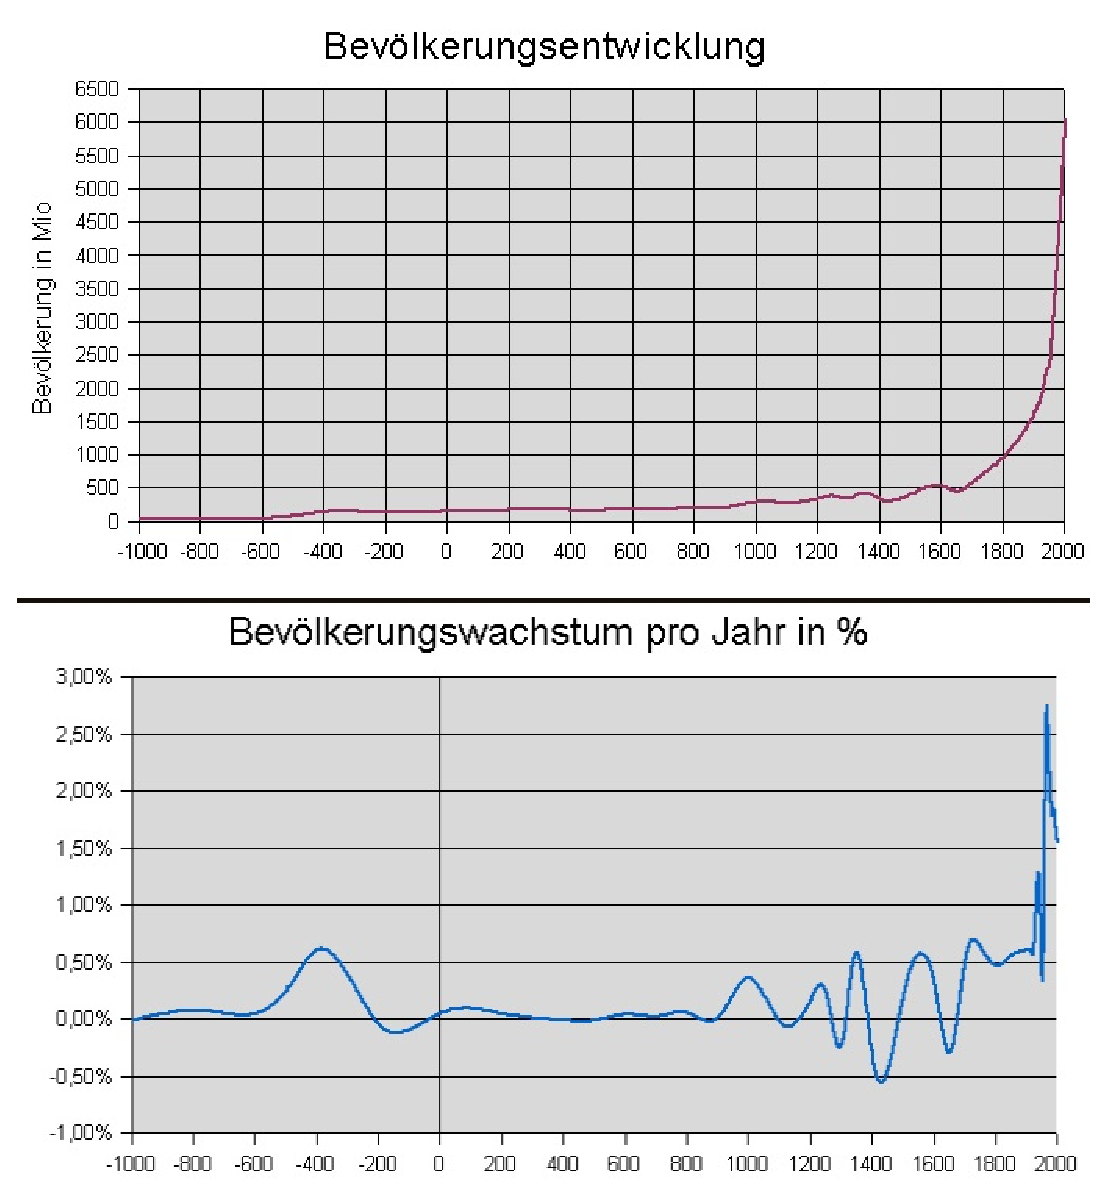
\includegraphics{../_database/Bilder/Bild24-1.eps}}
				\begin{tiny}Quelle: https://upload.wikimedia.org/wikipedia/commons/8/8a/World-pop-hist-de-2.png\end{tiny}
								
				\begin{scriptsize}Abbildung 1\end{scriptsize}
				\end{center}
				
				\meinlr{\resizebox{1\linewidth}{!}{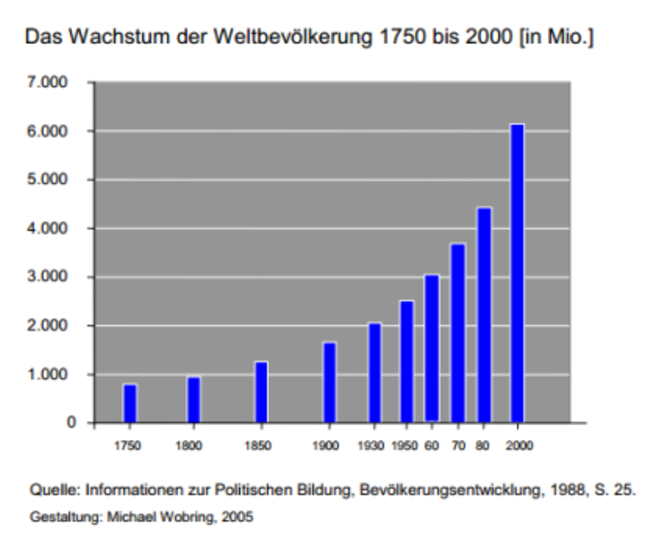
\includegraphics{../_database/Bilder/Bild24-2.eps}}
								\begin{center}\begin{scriptsize}Abbildung 2\end{scriptsize}\end{center}}{\resizebox{1.4\linewidth}{!}{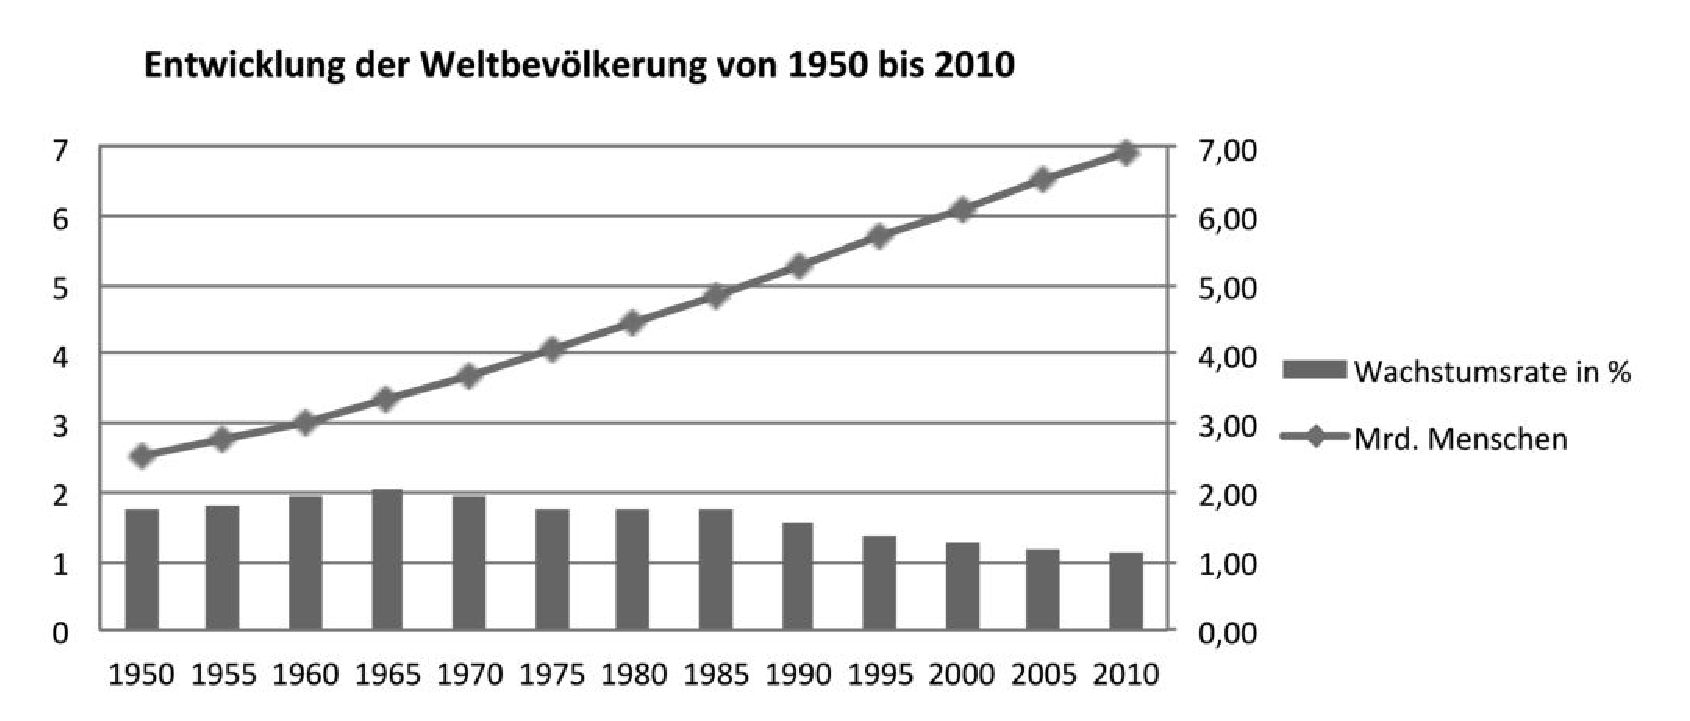
\includegraphics{../_database/Bilder/Bild24-3.eps}}
								\begin{center}\begin{scriptsize}Abbildung 3\end{scriptsize}\end{center}}\leer
								
				\begin{scriptsize}				
				\begin{tabular}{|C{1.7cm}|C{1.7cm}|C{1.7cm}|C{1.7cm}|C{1.7cm}|C{1.7cm}|C{1.7cm}|}\hline
				Jahr&Afrika&Asien&Europa&Lateinamerika&Nordamerika&Ozeanien\\ \hline
				1900&133&925&430&74&82&6\\ \hline
				1950&227&1\,403&547&167&172&13\\ \hline
				1975&419&2\,379&676&323&242&21\\ \hline
				2000&819&3\,698&727&521&319&31\\ \hline				
				\end{tabular}
				\end{scriptsize}

\subsection{Aufgabenstellung:}
\begin{enumerate}
	\item Ermittle anhand der Abbildungen, um wie viele Menschen die Weltbevölkerung von 1600 bis 18000 zugenommen hat!
	
	Nenne zwei Zeiträume, in denen die Weltbevölkerung mindesten 100 Jahre lang abgenommen hat, und begründe ihre Antwort!
	
	\item Die Weltbevölkerung hat von 1930 bis 1980 annähernd exponentiell zugenommen. Berechne unter dieser Annahme für diesen Zeitraum die jährliche Wachstumsrate auf Zehntelprozent genau!
	
	\item Begründe anhand der jährlichen Wachstumsraten aus Abbildung 3, warum die Entwicklung der Weltbevölkerung von 1950 bis 2010 nicht durch eine Exponentialfunktion beschrieben werden kann!
	
Bei konstanter Zunahme der Bevölkerungszahl ab 2010 wird für das Jahr 2050 eine Bevölkerungszahl von 10,4 Milliarden prognostiziert.\\
Berechne, von welcher jährlichen Zunahme bei dieser Prognose ausgegangen wird!
Gib die jährliche Zunahme in Millionen Menschen an!

\item Angenommen, die absoluten Zahlen der Bevölkerungsentwicklung der Kontinente und
Subkontinente im Zeitraum von 1900 bis 2000 werden in einem Säulendiagramm mit
linearer Skalierung dargestellt.\\
Begründe, warum die starke Bevölkerungszunahme in Ozeanien von 1900 bis 2000
in einem solchen Diagramm nicht erkennbar ist!

Gegeben sind fünf Aussagen zur Bevölkerungsentwicklung nach Kontinenten und Subkontinenten von 1900 bis 2000.\\
Kreuze die zutreffende(n) Aussage(n) an!\leer

\multiplechoice[5]{  %Anzahl der Antwortmoeglichkeiten, Standard: 5
				L1={Die Bevölkerung Asiens hat sich im 20. Jahrhundert annähernd
vervierfacht.},   %1. Antwortmoeglichkeit 
				L2={Seit Beginn des 20. Jahrhunderts lebten in Lateinamerika mehr
Menschen als in Nordamerika.},   %2. Antwortmoeglichkeit
				L3={Im Zeitraum von 1975 bis 2000 war die relative Bevölkerungszu-
nahme in Afrika am größten.},   %3. Antwortmoeglichkeit
				L4={In Europa war die Bevölkerungszunahme von 1975 bis 2000 ge-
ringer als von 1950 bis 1975.},   %4. Antwortmoeglichkeit
				L5={1950 lebten in Europa und Amerika zusammen bereits mehr als
eine Milliarde Menschen.},	 %5. Antwortmoeglichkeit
				L6={},	 %6. Antwortmoeglichkeit
				L7={},	 %7. Antwortmoeglichkeit
				L8={},	 %8. Antwortmoeglichkeit
				L9={},	 %9. Antwortmoeglichkeit
				%% LOESUNG: %%
				A1=1,  % 1. Antwort
				A2=3,	 % 2. Antwort
				A3=4,  % 3. Antwort
				A4=0,  % 4. Antwort
				A5=0,  % 5. Antwort
				}
						\end{enumerate}\leer
				
\antwort{\subsection{Lösungserwartung:}
\begin{enumerate}
	\item Zunahme von 1600 bis 1800: ca. 500 Millionen Menschen
	
	Die Weltbevölkerung hat mindestens 100 Jahre lang abgenommen in [250 v. Chr.; 50 v. Chr.] (bzw. $[-250;-50]$) und $[1400;1500]$, da in diesen Zeitintervallen das jährliche Bevölkerungswachstum in \% negativ ist.
	
	\item $N(t)=N_0\cdot a^t$\\
	$4,5=2\cdot a^50$\\
	$a\approx 1,016$, d.h. Zunahme um 1,6\,\% pro Jahr
	
	\item Bei einer exponentiellen Zunahme ist die jährliche Wachstumsrate konstant. Abbildung 3 zeigt, dass diese Voraussetzung im Zeitraum von 1950 bis 2010 nicht erfüllt ist.
	
	Konstante jährliche Zunahme von 2010 bis 2050:\\
	$\frac{10,4-6,9}{40}=0,0874$ Milliarden = 87,5 Millionen
	
	\item Da die Bevölkerungszahl Ozeaniens von 1900 bis 2000 jeweils weniger als 1\,\% der
Bevölkerungszahl Asiens betrug, sind die entsprechenden Säulen für Ozeanien sehr
niedrig (Höhe fast null).\\
Daher ist die Verfünffachung der Bevölkerungszahl Ozeaniens nicht erkennbar.

Lösung Multiple Choice siehe oben
			\end{enumerate}}
		\end{langesbeispiel}